\documentclass{beamer}

\usetheme{Copenhagen}
\usepackage[slovene]{babel}
\usepackage{ragged2e}
\usepackage{graphicx}

\title{1. domača naloga}
\subtitle{Napredna računalniška orodja}
\author{Igor Bojić}
\institute{Fakulteta za strojništvo}
\date{23.10.2023}
\logo{
\includegraphics[height=1.5cm]{fs logo.png}}

\begin{document}

\frame{\titlepage}
\begin{frame}
    \frametitle{Kazalo vsebine}
    \tableofcontents
\end{frame}
  
\AtBeginSection[]
{
  \begin{frame}
    \frametitle{Kazalo}
    \tableofcontents[currentsection]
  \end{frame}
}

\section{Git}
\begin{frame}
\frametitle{Github}
\justifying
V github sem naložil domačo nalogo, saj je repozitorij javen in majo do njega dostop vsi. V repozitorij sem povabil še kolega, ki je dopolnil določene lastnosti grafa. S tem lahko isto datoteko spreminjava oba, ostali pa lahko le opazujejo in ne morejo spreminjati datotek brez privolitve in sprejetja v repozitorij.
\end{frame}

\section{Beamer}

\begin{frame}
\frametitle{Predstavitev v Beamerju}
\justifying
V programu latex sem s pomočjo paketa Beamer izdelal ustrezno prezentacijo, kjer sem predstavil kaj vse sem v sklopu prve domače naloge naredil. To sem prikazal tudi z ustreznim kazalom 
\end{frame}


\section{Matlab}

\begin{frame}
\frametitle{Funkcijske in programske datoteke}

Definirali smo funkcijsko datoteko, ki mora imeti enak ime kot je poimenovana funkcija. Definiral sem dve prazni matriki, v kateri so se shranjevali podatki koordinat x in y, ob definiranem pogoju da je vsota kvadratov manjša od  kvadrata radija krožnice. Za tem sem definiral še:
\begin{itemize}
    \item Programsko datoteko.
    \begin{itemize}
        \item V programski datoteki sem najprej določil število točk, ki jih bomo izrisali-to je 10000.
        \end{itemize}
    \item Anonimno funkcijo, kjer sem definiral krožnico.
    \item Graf, ki se izriše, ko poženem kodo.
    \item Funkcijo, ki nam izračuna vrednost $\pi$ in napako glede na dejansko vrednost. 
\end{itemize}
\end{frame}

\begin{frame}
\frametitle{Funkcijske in programske datoteke}
\justifying
To je končni graf, ko poženem celotno kodo v programu Matlab, z že definiranimi osmi, naslovom in legendo, kar je spremenila oseba, povabljena v repozitorij. 
\begin{figure}
    \centering
    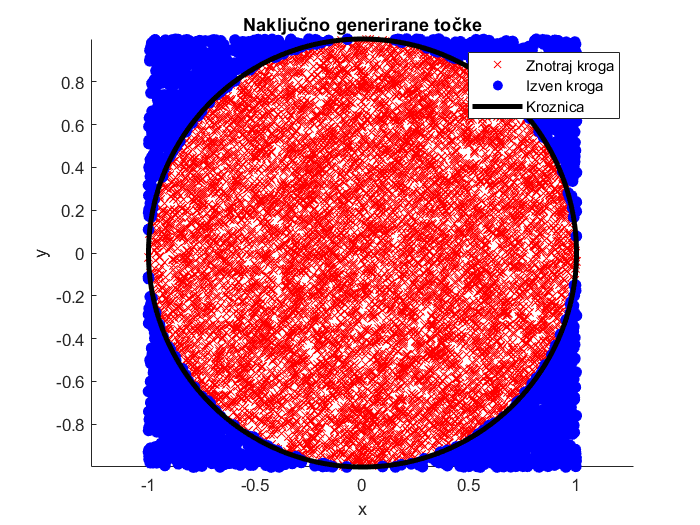
\includegraphics[width=0.6\textwidth]{graf.png}
    \caption{Graf z 10000 točkami.}
\end{figure}


\end{frame}

\end{document}
